%% V1.0
%% by Gabriel Garcia, gabrcg@gmail.com
%% This is a template for Udacity projects using IEEEtran.cls

%% Be Udacious!

\documentclass[10pt,journal,compsoc]{IEEEtran}

\usepackage[pdftex]{graphicx}    
\usepackage{cite}
\usepackage{hyperref}
\usepackage{subcaption}
\usepackage{wrapfig}
% \hyphenation{op-tical net-works semi-conduc-tor}

\begin{document}

\title{Deep RL Arm Manipulation}

\author{Lucas Wohlhart}

\markboth{Deep RL Arm Manipulation, Robotics Nanodegree Program, Udacity}%
{}
\IEEEtitleabstractindextext{%

%\begin{abstract}
%\end{abstract}

% Note that keywords are not normally used for peerreview papers.
\begin{IEEEkeywords}
Robot, Udacity, Reinforcement Learning, Object Manipulation
\end{IEEEkeywords}}

\maketitle
%\IEEEdisplaynontitleabstractindextext
%\IEEEpeerreviewmaketitle

%\IEEEPARstart{T}{he} 
\section{Introduction}
The goal of the DeepRL Project is the creation of an artificial agent operating a 3DoF robot manipulator arm to solve the task of touching a target can positioned in front of it. The base of the arm rotates around the z-axis and the two joints linking the serial arm segments to the base share the same rotation axis perpendicular to the z-axis.
The agent is tasked with controlling the joints such that it touches the can in front of it based on an image provided by a camera positioned next to the manipulators workspace. The control task at hand therefore falls into the category of visual servoing. The experimental setup is depicted in Fig.~\ref{fig:deep_rl_arm}.

\begin{figure}[htbp]
    \begin{center}
      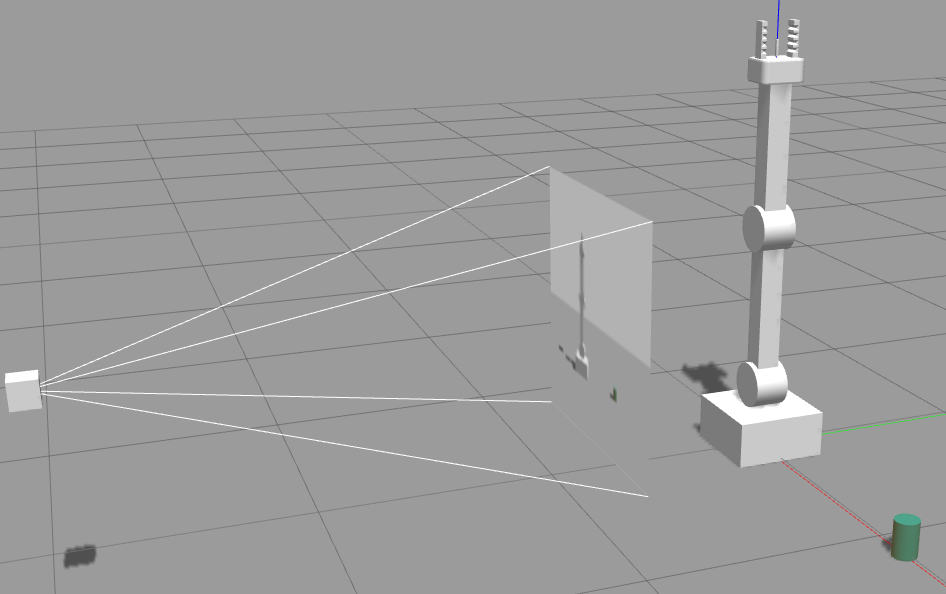
\includegraphics[width=0.6\textwidth]{img/deep_rl_arm}
    \end{center}
    \caption{Robot manipulator setup}
    \label{fig:deep_rl_arm}
\end{figure}
In task 1 of the project the entire arm of the manipulator is counted as valid collision target and an accuracy of 90\% successfull touches over at least 100 attempts has to be achieved.

In task 2 only the base of the parallel jaw gripper attached to the endeffector is allowed to touch the can for a successfull run and the accuracy has to exceed 80\% out of more than 100 iterations.

For all the experiments the base joint is locked, reducing the task to two degrees of freedom.

The agent could be set up to either operate on joint positions or joint velocities as control parameters.
The controlling agent has to choose between increasing or decreasing either of the two joints position/velocity. This yields 4 available actions the agent has to choose from at each time step, based on its policy and the provided input image state.

Through the use of reinforcement learning techniques the problem of training the agent can be solved by repeatedly letting it try to deduce actions based on the image and reward intended behaviour while penalizing erroneous actions.



%Have any part of the robot arm touch the object of interest, with at least a 90% accuracy for a minimum of 100 runs.
%The student should complete all tasks specified in the Classroom, with the end objective of the robot arm touching the object with at least a 90% accuracy for a minimum of 100 runs.
%Have only the gripper base of the robot arm touch the object, with at least a 80% accuracy for a minimum of 100 runs.
%The student should complete all tasks specified in the Classroom, with the end objective of the arm's gripper base touching the object with at least a 80% accuracy for a minimum of 100 runs.

\section{Reward Functions}  

The mechanisms used to reward the reinforcement learning agent are the following.
\begin{itemize}

    \item Whenever the agent sucessfully hits the can it receives REWARD\_WIN = 100 and the episode ends. In task 2 hitting the can with anything else but the gripper yields REWARD\_LOSS = -30.

    \item If the gripper ever hits the ground or the 100th simulation step is exceeded, the reward is REWARD\_LOSS = -30 and the episode is terminated.

    \item For each simulation step the average motion of the endeffector towards the goal ($avgGoalDelta$) is determined
    $$ avgGoalDelta \leftarrow \alpha * avgGoalDelta + (1 - \alpha) * distDelta $$
    where smoothing factor $\alpha = 0.2$ and $distDelta$ is the difference in endeffector-to-goal-distances of two consecutive steps.

    The resulting intermediate reward  that is issued every timestep is then comprised of a scaled motion based REWARD\_GOAL\_APPROACHING = 20 and a very small constant penalty of REWARD\_TIME\_PENALTY = -0.1.
    $$ reward = avgGoalDelta * 20 - 0.1 $$
    This yields positive rewards for average motion of the endeffector towards the goal.

\end{itemize}
%Explain the reward functions that you created.
%Brief explanation of each reward function and associated reward values. The writeup should also include what type of joint control was implemented.

\section{Hyperparameters}  
%Specify the hyperparameters that you selected for each objective, and explain the reasoning behind the selection.
%Student should explain the choice of hyperparameters for both objectives.

\begin{figure}[thpb]
    \centering
    \begin{tabular}{|c|c|}\hline
        INPUT\_WIDTH  & 64  \\ \hline
        INPUT\_HEIGHT & 64  \\ \hline
        OPTIMIZER & RMSprop  \\ \hline
        LEARNING\_RATE & 0.05 \\ \hline
        REPLAY\_MEMORY & 10000  \\ \hline
        BATCH\_SIZE & 128  \\ \hline
        USE\_LSTM & false  \\ \hline
        LSTM\_SIZE & \# \\ \hline
    \end{tabular}
\end{figure}

\section{Results}  

\begin{figure}[thpb]
    \centering
    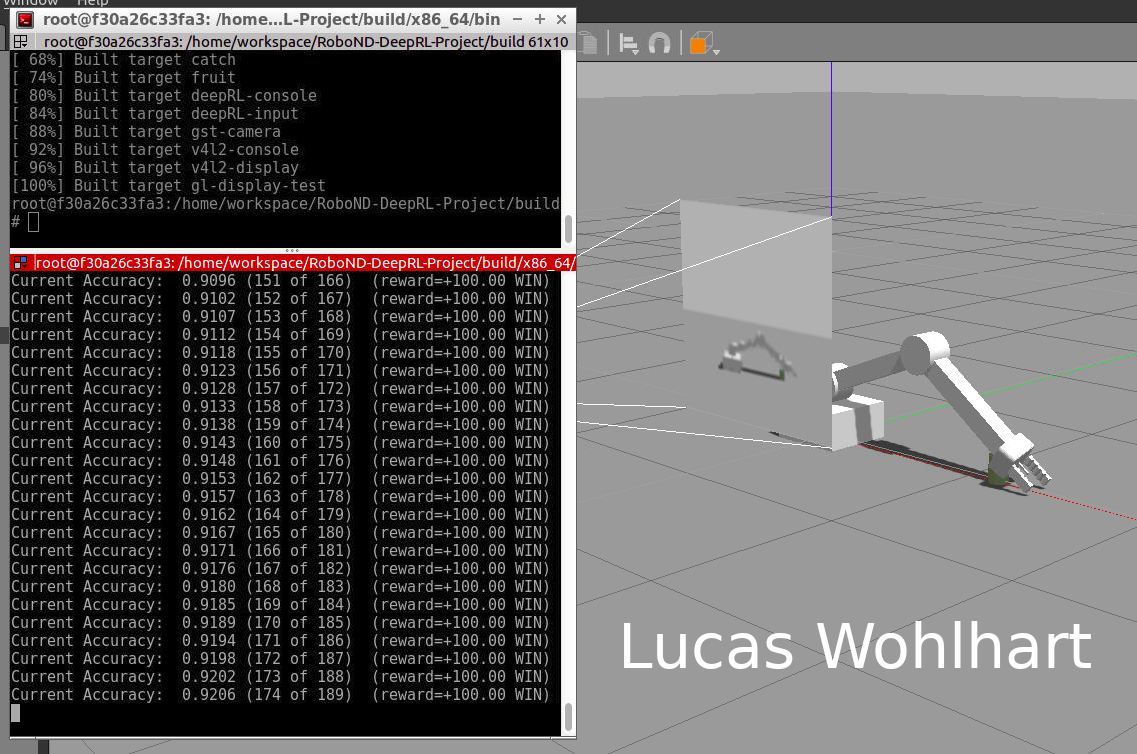
\includegraphics[width=0.75\linewidth]{img/task1_final.png}
    \caption{Task 1 final accuracy}
    \label{fig:task1_final}
\end{figure}

\begin{figure}[thpb]
    \centering
    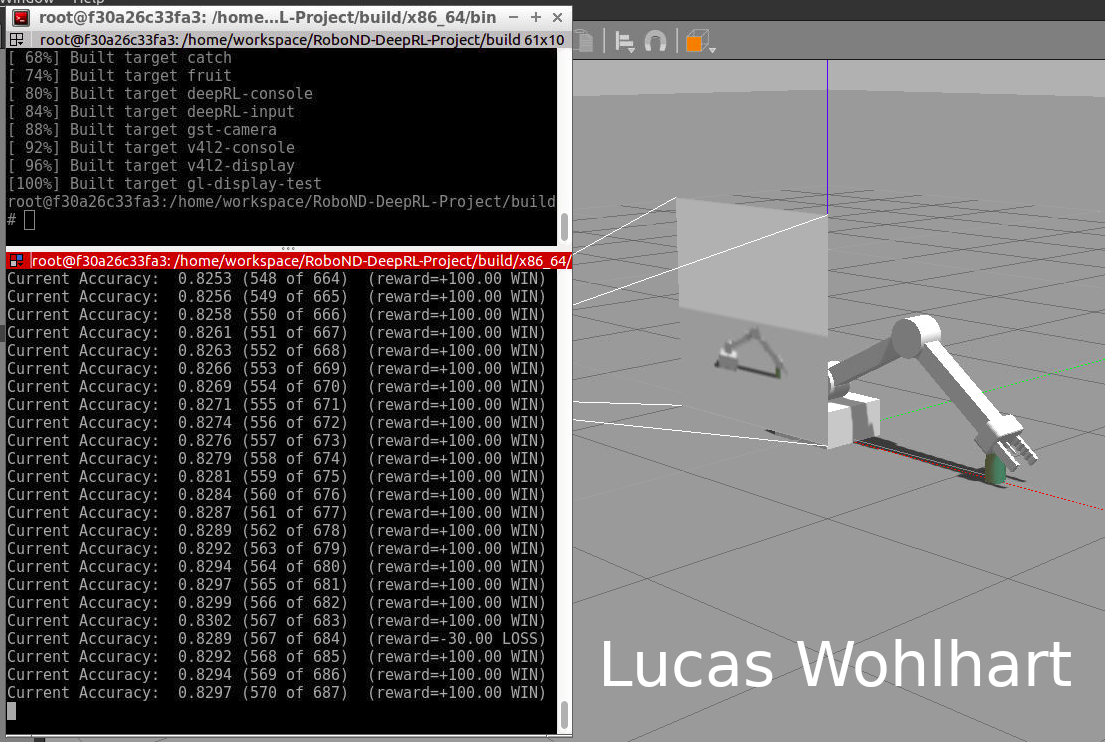
\includegraphics[width=0.75\linewidth]{img/task2_final.png}
    \caption{Task 2 final accuracy}
    \label{fig:task2_final}
\end{figure}

%Explain the results obtained for both objectives. Include discussion on the DQN agent's performance for both objectives. Include watermarked images, or videos of your results.
%Student should describe and briefly explain the results they achieved for both objectives. The discussion should also include their comments on the DQN agent's performance and if there were any shortcomings. Student should include either watermarked images of their results, or attach a video that displays the results and the arm in action.

\section{Future Work}  
%Briefly discuss how you can improve your current results.
%Student should discuss on what approaches they could take to improve their results.


% \bibliography{bib}
%\bibliographystyle{ieeetr}

\end{document}